\documentclass[tikz]{standalone}
\usepackage{tikz}
\usetikzlibrary{arrows}
\usetikzlibrary{3d}

\begin{document}
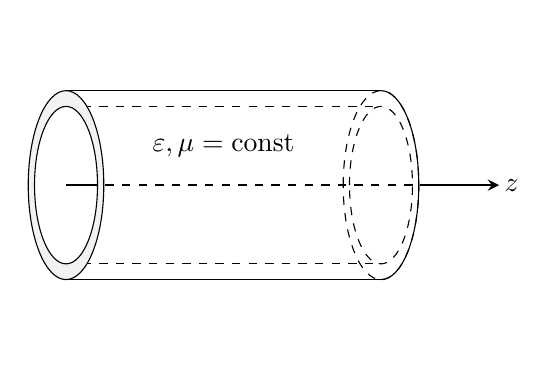
\begin{tikzpicture}[z={(1cm,0cm)}, y={(-0.4cm,-0cm)}, x={(0cm,1cm)}, scale=1,
    %Option for nice arrows
    >=stealth, %
    inner sep=0pt, outer sep=2pt,%
    axis/.style={thick,->},
    wave/.style={thick,color=#1,smooth},
    polaroid/.style={fill=black!60!white, opacity=0.3},
]
    % Colors
    \colorlet{darkgreen}{green!50!black}
    \colorlet{lightgreen}{green!80!black}
    \colorlet{darkred}{red!50!black}
    \colorlet{lightred}{red!80!black}

    \begin{scope}[canvas is yx plane at z=4]
        \draw[] (0,0,0) circle (1.2cm);
        % \draw[dashed] (0,0,0) circle (1cm);
        % \draw[fill=white] (0,0,0) circle (1cm);
    \end{scope}
    \begin{scope}[canvas is xz plane at y=0]
        \draw[draw=none,fill=white] (-2,4) rectangle (2,1);
    \end{scope}  
    \begin{scope}[canvas is yx plane at z=4]
        \draw[dashed] (0,0,0) circle (1cm);
        \draw[dashed] (0,0,0) circle (1.2cm);
        % \draw[fill=white] (0,0,0) circle (1cm);
    \end{scope}
    % Frame
    \coordinate (O) at (0, 0, 0);
    % \draw[axis] (O) -- +(1, 0,   0) node [above] {$x$};
    % \draw[axis] (O) -- +(-1, 0,   0) node [above] {$x$};
    % \draw[axis] (O) -- +(0,  1, 0) node [left] {$y$};
    % \draw[axis] (O) -- +(0,  -1, 0) node [left] {$y$};
    \draw[axis] (0,0,4+0.5) -- ++(0,  0,   1) node [right] {$z$};
    \draw[dashed,thick]  (0,0,0.5) -- (0,0,4+0.5);

    % \draw[thick,dashed] (-2,0,0) -- (O);



    \draw (1.2,0,0) -- ++(0,0,4);
    \draw[dashed] (1,0,0) -- ++(0,0,4);
    \draw[dashed] (-1,0,0) -- ++(0,0,4);
    \draw (-1.2,0,0) -- ++(0,0,4);
    \begin{scope}[canvas is yx plane at z=0]
        \draw[fill=black!5] (0,0,0) circle (1.2cm);
        \draw[fill=white] (0,0,0) circle (1cm);
    \end{scope}
    \draw[thick] (O) -- +(0,  0,   0.5*1/1.25);

    \draw (0.5,0,2) node {$\varepsilon,\mu=\mathrm{const}$};
%    %  % monochromatic incident light with electric field
%     \draw[wave=blue, op% acity=0.7, variable=\x, samples at={-2,-1.75,...,0}]
%         plot (\x, { cos(1.0*% \x r)*sin(2.0*\x r)}, { sin(1.0*\x r)*sin(2.0*\x r)})
%         plot (\x, {-cos(1.0*\% x r)*sin(2.0*\x r)}, {-sin(1.0*\x r)% *sin(2.0*\x r)});

%     \foreach \x in{-2% ,-1.75,...,0}{
%         \draw[color=blue, opacity=0.7,->]
%             (\x,0,0) -- (\x, { cos% (1.0*\x r)*sin(2.0*\x r)}, { sin(1.0*\x r)*sin(2.0*\x r)})
%             (\x,0,0) -- (\x, {-cos% (1.0*\x%  r)*sin(2.0*\x r)}, {-sin(1.0*\x r)*sin(2.0*\x r)});
%     }

%     \filldraw[polaroid] (0,-2% ,-1.5) -- (0,-2,1.5) -- (0,2,1.5) -- (0,2,-1.5) -- % (0,-2,-1.5)
%         node[below% , sloped, near end]{Polaroid};%

%     %Direction of%  polarization
%     \draw[thic% k,<->] (0,-1.75,-1) -- (0,-0.75,-1);

%     % Electric field%  vectors
%     \draw[wave=blue, variable=\x,samples at={0,0.25,...% ,6}]
%         plot (\x,{sin(2*\x r)},0)node[anchor=nort% h]{$\vec{E}$};

%     %Polarized l% ight between polaroid and thin section
%     \foreach \x in{0, 0.% 25,...,6}
%         \draw[color=blue,->] (\x,0,0) -- (\x,{sin(2*\x r)},0);

% % 
%     \draw (3,1,1) node [t% ext width=2.5cm, text cen% tered]{Polarized light};

%     %Crystal thin section
%     \begin{scope}[thick]
%      %    \draw (6,-2,-1.5) -- (6,-2,1.5) node [above, sloped, midway]{Cryst% al section}
%                 -- (6, 2, 1.5) -% - (6, 2, -1.5) -- cycle % First face
%        %      (6,  -2, -1.5) -- (6.2, -2,-1.5)
%       %       (6,   2, -1.5) -- (6.2,  2,-1.5)
%      %        (6,  -2,  1.5) -- (6.2, -2, 1.5)
%             (6,   2,  % 1.5) -- (6.2,  2, 1.5)
%             (6.2,-2, -1.5) -- (6.2,%  -2, 1.5) -- (6.2, 2, 1.5% ) 
%                 -- (6.2, 2, -1.5) -- cycle; % Second face

%         %Optical indices
%         \dra% w[darkred, ->]       (6.1, 0, 0) -- (6.1, 0.26,  0.966) node [right] {$n_{g}'$}% ; % index 1
%         \draw[darkred, dashed]   (6.1, 0, 0) -- (6.1,-0.26, -0.966); % index 1
%         \d% raw[darkgreen, ->]     (6.1, 0, 0) -- (6.1, 0.644,-0.173) node [right] {$n_{p}'% $}; % index 2
%   %       \draw[darkgreen, dashed] % (6.1, 0, 0) -- (6.1,-0.644, 0.173); % index 2
%     \end{scope}

%     % %Rays leaving thin section
%     \draw[wave=darkred,   variable=\x, samples at={6.2,6.45,...,12}] 
%    %      plot (\x, {0.26*0.26*sin(2*(\x-0.5) r)},  {0.966*0.26*sin(2*(\x-% 0.5) r)});  %n'g-oriented ray
%     \draw[wave=darkgreen, variable=\x, samples at={6.2,6.45,...,12}]
%  %        plot (\x, {0.966*0.966*sin(2*(\x-0.1) r)},{-0.26*0.966*sin(2*(\x-0.1) r)}); %n'p-ori% ented ray
%     \draw (10,1,1) node [te% xt width=2.5cm, text centered] {Polarized and dep% hased light};

%     \foreach \x in{6.2,6.45,...,12} {
%         \draw[color=darkgree% n, ->] (\x, 0, 0) --
%             (\x, {0.966*0.9% 66*sin(2*(\x-0.1) r)}, {-0.26*0.966*sin(2*(\x-0.1) r)});
%         \draw[color=dar% kred,  %  ->] (\x, 0, 0) --
%      %        (\x, {0.26*0.26*sin(2*(\x-0.5) r)}, {0.966*0.26*sin(2*(\x-0.5) r)});
% %     }

%     %Second polarization
%     \draw[polaroid]   (12, -2,  -1.5) -- (12, -2,   1.5% )  %Polarizing filter
%         node [above, sloped,midway] {Polaroid} -- (12, 2, 1.% 5) -- (12, 2, -1.5) -- cycle;
%     \dra% w[thick, <->] (12, -1.5,-0.5) -- (12, -1.5, 0.5); %Polarization directi% on

%     %Light leaving the second polaroid
%     \draw[wave=lightgreen,variable% =\x, samples at={12, 12.25,..., 14}]
%         plot (\x,{0}, {0.966*0.96% 6*0.26*sin(2*(\x-0.5) r)}); %n'g polarized ray
%     \draw[wave=lightred,  variabl% e=\x, samples at={12, 12.25,..., 14}]
%         plot (\x,{0}, {-0.26*0.966*sin(2*(\x-0.1) r)});      %n'p polari% zed ray

%     \node[align=justify, text width=14cm, anchor=north west, ysh% ift=-2mm] at (current bounding box.south west)
%         {Light behavior in a % petrographic microscope with light polarizing
%         device. Only one incident wavelength is shown (monochromatic light).
%         The magnetic field, perpendicular to the electric one, is not drawn.};
\end{tikzpicture}
\end{document}